\documentclass[10pt,a4paper]{article}

% Core formatting and typography
\usepackage[utf8]{inputenc}
\usepackage[T1]{fontenc}
\usepackage{lmodern}
\usepackage{amsmath,amssymb}
\usepackage{booktabs}
\usepackage{graphicx}
\usepackage{tabularx}
\usepackage{multicol}
\usepackage{microtype}
\usepackage[table]{xcolor}
\usepackage[margin=0.68in,top=0.65in,bottom=0.65in]{geometry}
\usepackage[colorlinks=true,linkcolor=blue!70!black,citecolor=blue!70!black,urlcolor=blue!70!black]{hyperref}

% Set graphicspath so figures resolve whether compiled from root or report/
\graphicspath{{../outputs/figures/}{outputs/figures/}}

% Custom macros
\newcommand{\INR}{\text{INR~}}
\newcommand{\Rs}{\text{Rs.~}}

% Compact spacing adjustments to ensure exact 1 section per page
\setlength{\parindent}{0pt}
\setlength{\emergencystretch}{1em}
\setlength{\parskip}{4pt}
\renewcommand{\arraystretch}{1.12}

\begin{document}

% ==============================================================================
% PAGE 1: SECTION 1 - THE QUESTION (20% Rubric Weight)
% ==============================================================================
\pagestyle{plain}
\pagenumbering{arabic}

\begin{center}
    {\Large \textbf{Optimisation of Food Grain Distribution from FCI Depots to District Warehouses in Gujarat}}\\[4pt]
    {\normalsize \textbf{CE 637 Infrastructure Systems: Planning and Management}}\\[2pt]
    {\small \textbf{Course Project, IIT Gandhinagar} $\;\vert\;$ \textbf{Authors:} Abhitej Singh Bhullar (Roll No.~23110009) \& Radhika Purohit (Roll No.~24110280) $\;\vert\;$ November 2026}
\end{center}
\vspace{-4pt}
\hrule
\vspace{6pt}

\section*{Section 1: The Question}
At the beginning of each month, the General Manager (Logistics \& Movement) at the Food Corporation of India (FCI) Gujarat Regional Office, in coordination with the Managing Director of the Gujarat State Civil Supplies Corporation Limited (GSCSCL), must decide how wheat and rice should move from storage depots to district warehouses so that households can receive their food grains through the public distribution system under the National Food Security Act (NFSA). In the simplified Gujarat network considered in this study, grain is available at four depots : Sabarmati, Chhani, Ghanteshwar and Gandhidham, and must be delivered to six districts: Ahmedabad, Surat, Vadodara, Rajkot, Banaskantha and Kutch. Together, these districts require 132,000 metric tonnes (MT) per month, comprising 90,000 MT of wheat and 42,000 MT of rice. Sending each district's requirement from its nearest depot may seem the obvious choice, but the nearest depot cannot always load enough grain. For example, Chhani can dispatch only 28,000 MT per month, while nearby Vadodara and Surat together require 55,000 MT, so other depots must help meet their demand. Those additional shipments may travel farther and increase the transport bill. The planner must track wheat and rice separately. Spare rice cannot fill a wheat order, and both grains use the same loading facilities. The challenge is therefore to decide how many tonnes of wheat and rice to send along each of the 24 depot-to-district routes so that every district receives its full monthly requirement at the lowest total transport and handling cost, without exceeding any depot's available stock or loading capacity.

\vspace{6pt}
\begin{center}
\fbox{
\begin{minipage}{0.96\textwidth}
\footnotesize \centering
\textbf{DEPOTS AND DISTRICT WAREHOUSES IN GUJARAT}\\
\vspace{2pt}
\resizebox{\textwidth}{!}{
\begin{tabular}{rcccl}
\textbf{FCI Depots} & & & & \textbf{GSCSCL District Warehouses}\\
\textbf{D1: Sabarmati (Ahmd)} [Cap: 45k MT; Stock: 35k W, 18k R] & $\xrightarrow{\hspace{1.2cm}}$ & $\dots$ & $\xrightarrow{\hspace{1.2cm}}$ & \textbf{W1: Ahmedabad} [Demand: 24k W, 10k R] (34k MT)\\
\textbf{D2: Chhani (Vadodara)} [Cap: 28k MT; Stock: 22k W, 12k R] & $\xrightarrow{\hspace{1.2cm}}$ & $\dots$ & $\xrightarrow{\hspace{1.2cm}}$ & \textbf{W2: Surat} [Demand: 22k W, 12k R] (34k MT)\\
\textbf{D3: Ghanteshwar (Rajkot)} [Cap: 30k MT; Stock: 25k W, 10k R] & $\xrightarrow{\hspace{1.2cm}}$ & $\dots$ & $\xrightarrow{\hspace{1.2cm}}$ & \textbf{W3: Vadodara} [Demand: 14k W, 7k R] (21k MT)\\
\textbf{D4: Gandhidham (Kutch)} [Cap: 38k MT; Stock: 30k W, 15k R] & $\xrightarrow{\hspace{1.2cm}}$ & $\dots$ & $\xrightarrow{\hspace{1.2cm}}$ & \textbf{W4: Rajkot} [Demand: 13k W, 5k R] (18k MT)\\
& & & $\xrightarrow{\hspace{1.2cm}}$ & \textbf{W5: Banaskantha} [Demand: 11k W, 5k R] (16k MT)\\
\textit{Shared Loading Bays and Weighbridges} & & & $\xrightarrow{\hspace{1.2cm}}$ & \textbf{W6: Kutch/Bhuj} [Demand: 6k W, 3k R] (9k MT)\\
\end{tabular}
}
\end{minipage}
}
\end{center}

\vspace{6pt}
\textbf{Table 1.1: Depot Stocks, Loading Limits and District Demand}
\vspace{-4pt}
\begin{table}[h!]
\centering
\resizebox{\textwidth}{!}{
\begin{tabular}{lllcccccl}
\toprule
\textbf{Node} & \textbf{Facility Name} & \textbf{District} & \textbf{Role} & \textbf{Latitude} & \textbf{Longitude} & \textbf{Wheat (MT)} & \textbf{Rice (MT)} & \textbf{Monthly Loading Limit or Demand} \\
\midrule
\textbf{D1} & FSD Sabarmati (Ahmd) & Ahmedabad & Supply Depot & 23.0760$^\circ$N & 72.5800$^\circ$E & 35,000 & 18,000 & Dispatch Cap: 45,000 MT (Stock: 53,000 MT) \\
\textbf{D2} & FSD Chhani (Vadodara) & Vadodara & Supply Depot & 22.3580$^\circ$N & 73.1650$^\circ$E & 22,000 & 12,000 & Dispatch Cap: 28,000 MT (Stock: 34,000 MT) \\
\textbf{D3} & FSD Ghanteshwar (Rajkot) & Rajkot & Supply Depot & 22.3450$^\circ$N & 70.7550$^\circ$E & 25,000 & 10,000 & Dispatch Cap: 30,000 MT (Stock: 35,000 MT) \\
\textbf{D4} & FSD Gandhidham (Kutch) & Kutch & Supply Depot & 23.0753$^\circ$N & 70.1337$^\circ$E & 30,000 & 15,000 & Dispatch Cap: 38,000 MT (Stock: 45,000 MT) \\
\midrule
\textbf{W1} & Ahmedabad district HQ & Ahmedabad & Warehouse & 23.0225$^\circ$N & 72.5714$^\circ$E & 24,000 & 10,000 & Demand: 34,000 MT (25.76\%) \\
\textbf{W2} & Surat district HQ & Surat & Warehouse & 21.1702$^\circ$N & 72.8311$^\circ$E & 22,000 & 12,000 & Demand: 34,000 MT (25.76\%) \\
\textbf{W3} & Vadodara district HQ& Vadodara & Warehouse & 22.3072$^\circ$N & 73.1812$^\circ$E & 14,000 & 7,000 & Demand: 21,000 MT (15.91\%) \\
\textbf{W4} & Rajkot district HQ & Rajkot & Warehouse & 22.3039$^\circ$N & 70.8022$^\circ$E & 13,000 & 5,000 & Demand: 18,000 MT (13.64\%) \\
\textbf{W5} & Palanpur district HQ & Banaskantha & Warehouse & 24.1724$^\circ$N & 72.4346$^\circ$E & 11,000 & 5,000 & Demand: 16,000 MT (12.12\%) \\
\textbf{W6} & Bhuj district HQ& Kutch & Warehouse & 23.2420$^\circ$N & 69.6669$^\circ$E & 6,000 & 3,000 & Demand: 9,000 MT (6.82\%) \\
\midrule
\multicolumn{4}{l}{\textbf{Total Available Stock / District Demand}} & & & \textbf{112,000 / 90,000} & \textbf{55,000 / 42,000} & \textbf{System Cap: 141,000 / Demand: 132,000 MT} \\
\bottomrule
\end{tabular}
}
\end{table}


\vfill
\begin{flushright}
\footnotesize \textit{Page 1 of 7}
\end{flushright}

\newpage

% ==============================================================================
% PAGE 2: SECTION 2 - THE MODEL (25% Rubric Weight)
% ==============================================================================
\section*{Section 2: The Model}


\subsection*{1. Mathematical Formulation}
\textbf{Sets and Indices:} $i \in I = \{1, 2, 3, 4\}$ (FCI Depots), $j \in J = \{1, \dots, 6\}$ (District Warehouses), $k \in K = \{1, 2\}$ (1: Wheat, 2: Rice).\\[2pt]
\textbf{Decision Variables:} $x_{ijk} \ge 0$ denotes metric tonnes (MT) of commodity $k$ dispatched from depot $i$ to district $j$ per month ($4 \times 6 \times 2 = \mathbf{48}$ variables).\\[2pt]
\textbf{Objective Function:} Minimize scenario monthly freight haulage and handling expenditure:
\begin{equation}
\min Z = \sum_{i=1}^4 \sum_{j=1}^6 \sum_{k=1}^2 c_{ij} x_{ijk} = \sum_{i=1}^4 \sum_{j=1}^6 c_{ij} (x_{ij1} + x_{ij2})
\end{equation}
where $c_{ij} = \alpha + \beta \cdot d_{ij} = 100.00 + 2.50 \cdot d_{ij}$ [INR/MT] is the linear freight cost model, with route rates rounded to two decimal places.\\[2pt]
\textbf{System Constraints (24 Linear Inequalities):}
\begin{align}
\text{1. Depot Commodity Stock Limits (8):} \quad & \sum_{j=1}^6 x_{ijk} \le S_{ik} \quad \forall i \in \{1, \dots, 4\}, \; \forall k \in \{1, 2\} \\
\text{2. District Demand Requirements (12):} \quad & \sum_{i=1}^4 x_{ijk} \ge D_{jk} \quad \forall j \in \{1, \dots, 6\}, \; \forall k \in \{1, 2\} \\
\text{3. Depot Dispatch Capacity Coupling (4):} \quad & \sum_{k=1}^2 \sum_{j=1}^6 x_{ijk} \le C_i \quad \forall i \in \{1, \dots, 4\} \\
\text{4. Non-Negativity Restrictions (48):} \quad & x_{ijk} \ge 0 \quad \forall i \in I, \; j \in J, \; k \in K
\end{align}

\vspace{-4pt}
\textbf{Table 2.1: Road Distances $d_{ij}$ (km) and Transport Cost per Tonne $c_{ij}$ (INR/MT)}
\begin{table}[h!]
\centering
\resizebox{\textwidth}{!}{
\begin{tabular}{lcccccc}
\toprule
\textbf{Origin Depot} & \textbf{W1 (Ahmedabad)} & \textbf{W2 (Surat)} & \textbf{W3 (Vadodara)} & \textbf{W4 (Rajkot)} & \textbf{W5 (Banaskantha)} & \textbf{W6 (Kutch/Bhuj)} \\
\midrule
\textbf{D1: Sabarmati (Ahmd)} & 6.7 km (\INR 116.85) & 257.4 km (\INR 743.55) & 122.3 km (\INR 405.75) & 220.3 km (\INR 650.83) & 140.2 km (\INR 450.50) & 356.9 km (\INR 992.32) \\
\textbf{D2: Chhani (Vadodara)} & 102.6 km (\INR 356.42) & 154.9 km (\INR 487.20) & 7.5 km (\INR 118.80) & 274.8 km (\INR 786.88) & 253.3 km (\INR 733.35) & 450.5 km (\INR 1226.25) \\
\textbf{D3: Ghanteshwar (Rajkot)} & 222.4 km (\INR 656.12) & 429.8 km (\INR 1174.48) & 290.0 km (\INR 825.08) & 8.5 km (\INR 121.32) & 326.6 km (\INR 916.58) & 239.2 km (\INR 698.10) \\
\textbf{D4: Gandhidham (Kutch)} & 356.7 km (\INR 991.75) & 564.0 km (\INR 1510.10) & 424.3 km (\INR 1160.68) & 199.9 km (\INR 599.65) & 320.3 km (\INR 900.70) & 57.6 km (\INR 244.05) \\
\bottomrule
\end{tabular}
}
\end{table}

\vspace{-4pt}

\subsection*{2. Why the Shared Loading Limit Matters}
Because shipping grain costs money on every route, the solver will never ship more grain to a district than it asks for. Every district receives its exact requirement. Without Constraint (3), we could plan wheat and rice separately in two tables, one for each grain. But depots use the same loading bays, labour crews and weighbridges for both grains. Each depot can load less in a month than it holds in stock. Chhani, for example, holds 34,000 MT but can load only 28,000 MT per month. Wheat and rice must therefore share that limit. The lowest-cost plan uses all the loading capacity at Sabarmati, Chhani and Ghanteshwar, while Gandhidham has 9,000 MT of spare capacity.

\subsection*{3. Modeling Assumptions}
\begin{itemize}\setlength{\itemsep}{1pt}\setlength{\parskip}{0pt}
\item \textbf{Uniform Grain Quality.} All wheat and rice is of standard fair average quality, so grain from any depot can satisfy any district.
\item \textbf{Single Average Month.} We plan for one standard 30-day month rather than tracking day-by-day inventory changes.
\item \textbf{Linear Transport Cost.} Shipping cost per tonne rises with road distance at a fixed rate. Handling costs Rs.~100 per tonne and transport costs Rs.~2.50 per tonne-km.
\item \textbf{District-Level Grouping.} Demand from individual towns and ration shops is grouped at the main district warehouse.
\item \textbf{Zero Transit Loss.} We assume no grain is spilled or spoiled during highway transport.
\item \textbf{Direct Point-to-Point Delivery.} Trucks go from an FCI depot to a district warehouse without stopping at intermediate hubs.
\end{itemize}

\vfill
\begin{flushright}
\footnotesize \textit{Page 2 of 7}
\end{flushright}

\newpage

% ==============================================================================
% PAGE 3: SECTION 3 - THE METHOD (25% Rubric Weight)
% ==============================================================================
\section*{Section 3: The Method}


\subsection*{1. Why Linear Programming and Two-Phase Simplex Fit This Problem}
\textbf{Why linear programming?} Cost, stock use, district deliveries and depot loading are all sums of the tonnes shipped, with a fixed cost per tonne on each route. Standard transportation methods such as MODI and Stepping-Stone are designed for a single product. Using one table for wheat and another for rice would miss the loading limit the two grains share. Linear programming includes that limit directly and finds the lowest-cost schedule that meets all the rules.

\textbf{Why two phases?} Simplex needs a valid starting schedule, called a basic feasible solution. With only upper limits, sending nothing can give us a place to start. Here, sending nothing leaves all 132,000 MT of district demand unmet. Phase I finds a schedule that meets demand and stays within the depot limits. Phase II lowers its cost.


\subsection*{2. Converting the Problem into Standard Simplex Form}
Simplex works with equations and nonnegative variables. The 48 shipment variables stay in the model. We add 8 stock slacks $s^S_{ik}$ for unused grain and 4 loading slacks $s^C_i$ for unused capacity. For each of the 12 demand limits, we subtract a surplus $e_{jk}$ for extra deliveries and add an artificial variable $a_{jk}$ to start Phase I.

\begin{center}
{\small\textbf{Standard form for Phase I: 24 equations and 84 variables}\par\smallskip}
{\footnotesize
\setlength{\tabcolsep}{5pt}
\begin{tabular}{lcccccc}
\toprule
\textbf{Constraint} &
\shortstack{\textbf{Shipments}\\$x_{ijk}$ (48)} &
\shortstack{\textbf{Stock slack}\\$s^S_{ik}$ (8)} &
\shortstack{\textbf{Loading slack}\\$s^C_i$ (4)} &
\shortstack{\textbf{Demand surplus}\\$e_{jk}$ (12)} &
\shortstack{\textbf{Artificial}\\$a_{jk}$ (12)} &
\textbf{Equals} \\
\midrule
Stock (8) & $\sum_j x_{ijk}$ & $+s^S_{ik}$ & & & & $S_{ik}$ \\
Loading (4) & $\sum_{j,k} x_{ijk}$ & & $+s^C_i$ & & & $C_i$ \\
Demand (12) & $\sum_{i} x_{ijk}$ & & & $-e_{jk}$ & $+a_{jk}$ & $D_{jk}$ \\
\bottomrule
\end{tabular}}
\end{center}
Each row shows the terms on the left of its equation. With $x_{ijk}=0$ and $e_{jk}=0$, the starting values $s^S_{ik}=S_{ik}$, $s^C_i=C_i$ and $a_{jk}=D_{jk}$ balance all 24 equations. For example, a 10 MT wheat requirement starts with $a_{jk}=10$. Phase I replaces that temporary amount with shipments.

\subsection*{3. How the Solver Reached the Optimal Answer}
\textbf{Phase I. Find a feasible schedule.} The first objective is to minimise $W=\sum_{j,k}a_{jk}$. It starts at 132,000 MT. The solver uses the minimum-ratio test to keep the variables nonnegative and Bland's rule to select an entering variable and break ties. After \textbf{28 steps (pivots)}, $W=0$. Since all artificial variables are nonnegative, each is zero and the shipments meet the original constraints.

\textbf{Phase II. Minimise transport cost.} The solver removes the artificial columns and writes the rupee cost objective for the feasible basis from Phase I. It uses reduced costs to identify changes that could lower total cost while the basic variables adjust. After another 28 steps, no reduced cost is below $-10^{-9}$, the cutoff used to test for improvement. The run took \textbf{56 pivots in total} and reached a minimum monthly cost of \textbf{INR 5,69,82,720 (Rs.~5.70 crore)}.

\textbf{Independent check.} SciPy's \texttt{linprog} with the HiGHS dual simplex method gave the same minimum for the original 48-variable model, \textbf{INR 5,69,82,720.00}.

\vfill
\begin{flushright}
\footnotesize \textit{Page 3 of 7}
\end{flushright}

\newpage

% ==============================================================================
% PAGE 4: SECTION 4 - THE ANSWER (20% Rubric Weight)
% ==============================================================================
\section*{Section 4: The Answer}

\subsection*{1. The Lowest-Cost Monthly Plan}
The optimal plan meets the monthly demand of 132,000 MT at a total cost of \textbf{\INR 56,982,720.00} (\textbf{\Rs 5.6983 Crore}). The average cost is \textbf{\INR 431.69 per MT}, and total haulage work is \textbf{17.51 Million Tonne-km}.
\par Wheat and rice cost the same to ship on a given route. If two depots can exchange equal amounts of wheat and rice for the same district while following all shipment and stock limits, the total cost stays the same.

\vspace{-4pt}
\textbf{Table 4.1: Monthly Wheat and Rice Shipments}
\begin{table}[h!]
\centering
\resizebox{\textwidth}{!}{
\begin{tabular}{llccccccc}
\toprule
\textbf{Origin Supply Depot} & \textbf{Destination Warehouse} & \textbf{Distance (km)} & \textbf{Wheat (MT)} & \textbf{Rice (MT)} & \textbf{Total Flow (MT)} & \textbf{Unit Cost} & \textbf{Total Cost (INR)} & \textbf{Tonne-km} \\
\midrule
\textbf{D1: Sabarmati (Ahmd)} & \textbf{W1: Ahmedabad} & 6.74 & 24,000.0 & 10,000.0 & \textbf{34,000.0} & \INR 116.85 & \INR 3,972,900.00 & 229,160.0 \\
\textbf{D1: Sabarmati (Ahmd)} & \textbf{W2: Surat} & 257.42 & 3,000.0 & 8,000.0 & \textbf{11,000.0} & \INR 743.55 & \INR 8,179,050.00 & 2,831,620.0 \\
\textbf{D2: Chhani (Vadodara)} & \textbf{W2: Surat} & 154.88 & 7,000.0 & 0.0 & \textbf{7,000.0} & \INR 487.20 & \INR 3,410,400.00 & 1,084,160.0 \\
\textbf{D2: Chhani (Vadodara)} & \textbf{W3: Vadodara} & 7.52 & 14,000.0 & 7,000.0 & \textbf{21,000.0} & \INR 118.80 & \INR 2,494,800.00 & 157,920.0 \\
\textbf{D3: Ghanteshwar (Rajkot)} & \textbf{W2: Surat} & 429.79 & 12,000.0 & 0.0 & \textbf{12,000.0} & \INR 1,174.48 & \INR 14,093,760.00 & 5,157,480.0 \\
\textbf{D3: Ghanteshwar (Rajkot)} & \textbf{W4: Rajkot} & 8.53 & 13,000.0 & 5,000.0 & \textbf{18,000.0} & \INR 121.32 & \INR 2,183,760.00 & 153,540.0 \\
\textbf{D4: Gandhidham (Kutch)} & \textbf{W2: Surat} & 564.04 & 0.0 & 4,000.0 & \textbf{4,000.0} & \INR 1,510.10 & \INR 6,040,400.00 & 2,256,160.0 \\
\textbf{D4: Gandhidham (Kutch)} & \textbf{W5: Banaskantha} & 320.28 & 11,000.0 & 5,000.0 & \textbf{16,000.0} & \INR 900.70 & \INR 14,411,200.00 & 5,124,480.0 \\
\textbf{D4: Gandhidham (Kutch)} & \textbf{W6: Kutch (Bhuj)} & 57.62 & 6,000.0 & 3,000.0 & \textbf{9,000.0} & \INR 244.05 & \INR 2,196,450.00 & 518,580.0 \\
\midrule
\multicolumn{3}{l}{\textbf{MONTHLY TOTAL}} & \textbf{90,000.0} & \textbf{42,000.0} & \textbf{132,000.0} & \textbf{--} & \textbf{\INR 56,982,720.00} & \textbf{17,513,100.0} \\
\bottomrule
\end{tabular}
}
\end{table}

\vspace{-4pt}
\begin{figure}[h!]
\centering
\begin{minipage}{0.49\textwidth}
\centering
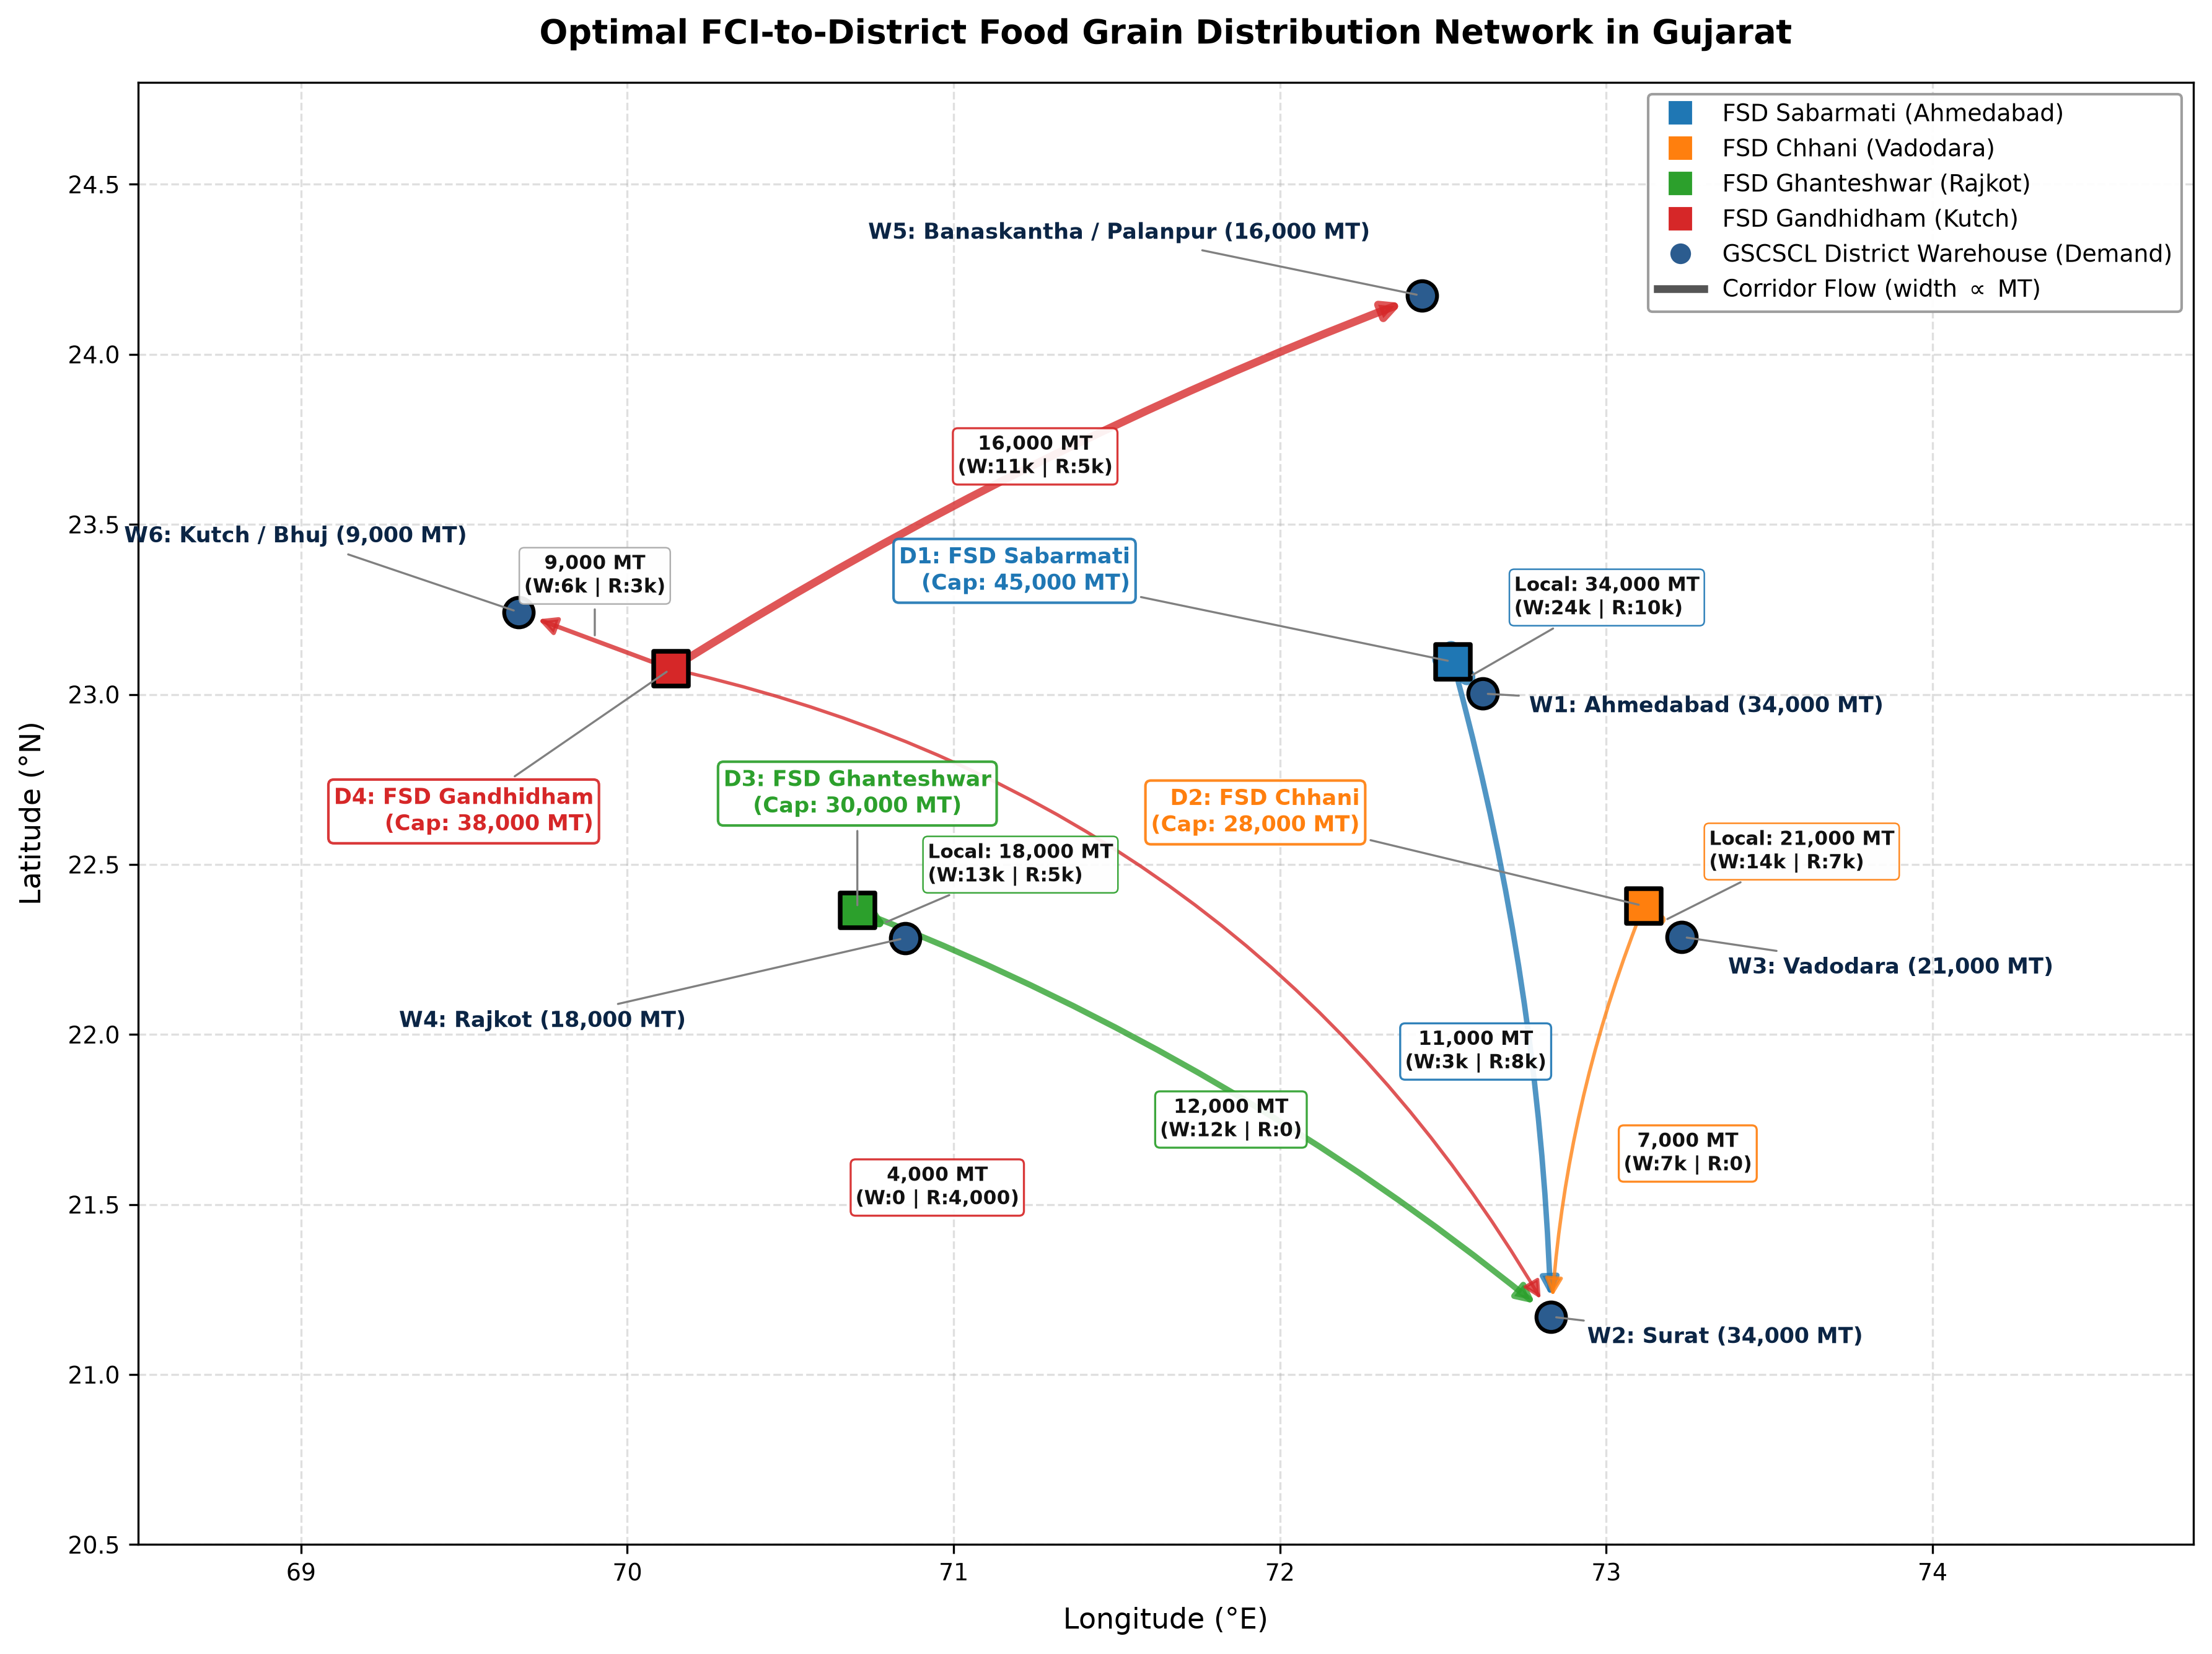
\includegraphics[width=\textwidth]{fig1_network_flow_map.png}\\
\vspace{-4pt}
\caption{\footnotesize Optimal Food Grain Network Flow Map (Line width $\propto$ tonnage).}
\end{minipage}\hfill
\begin{minipage}{0.49\textwidth}
\centering
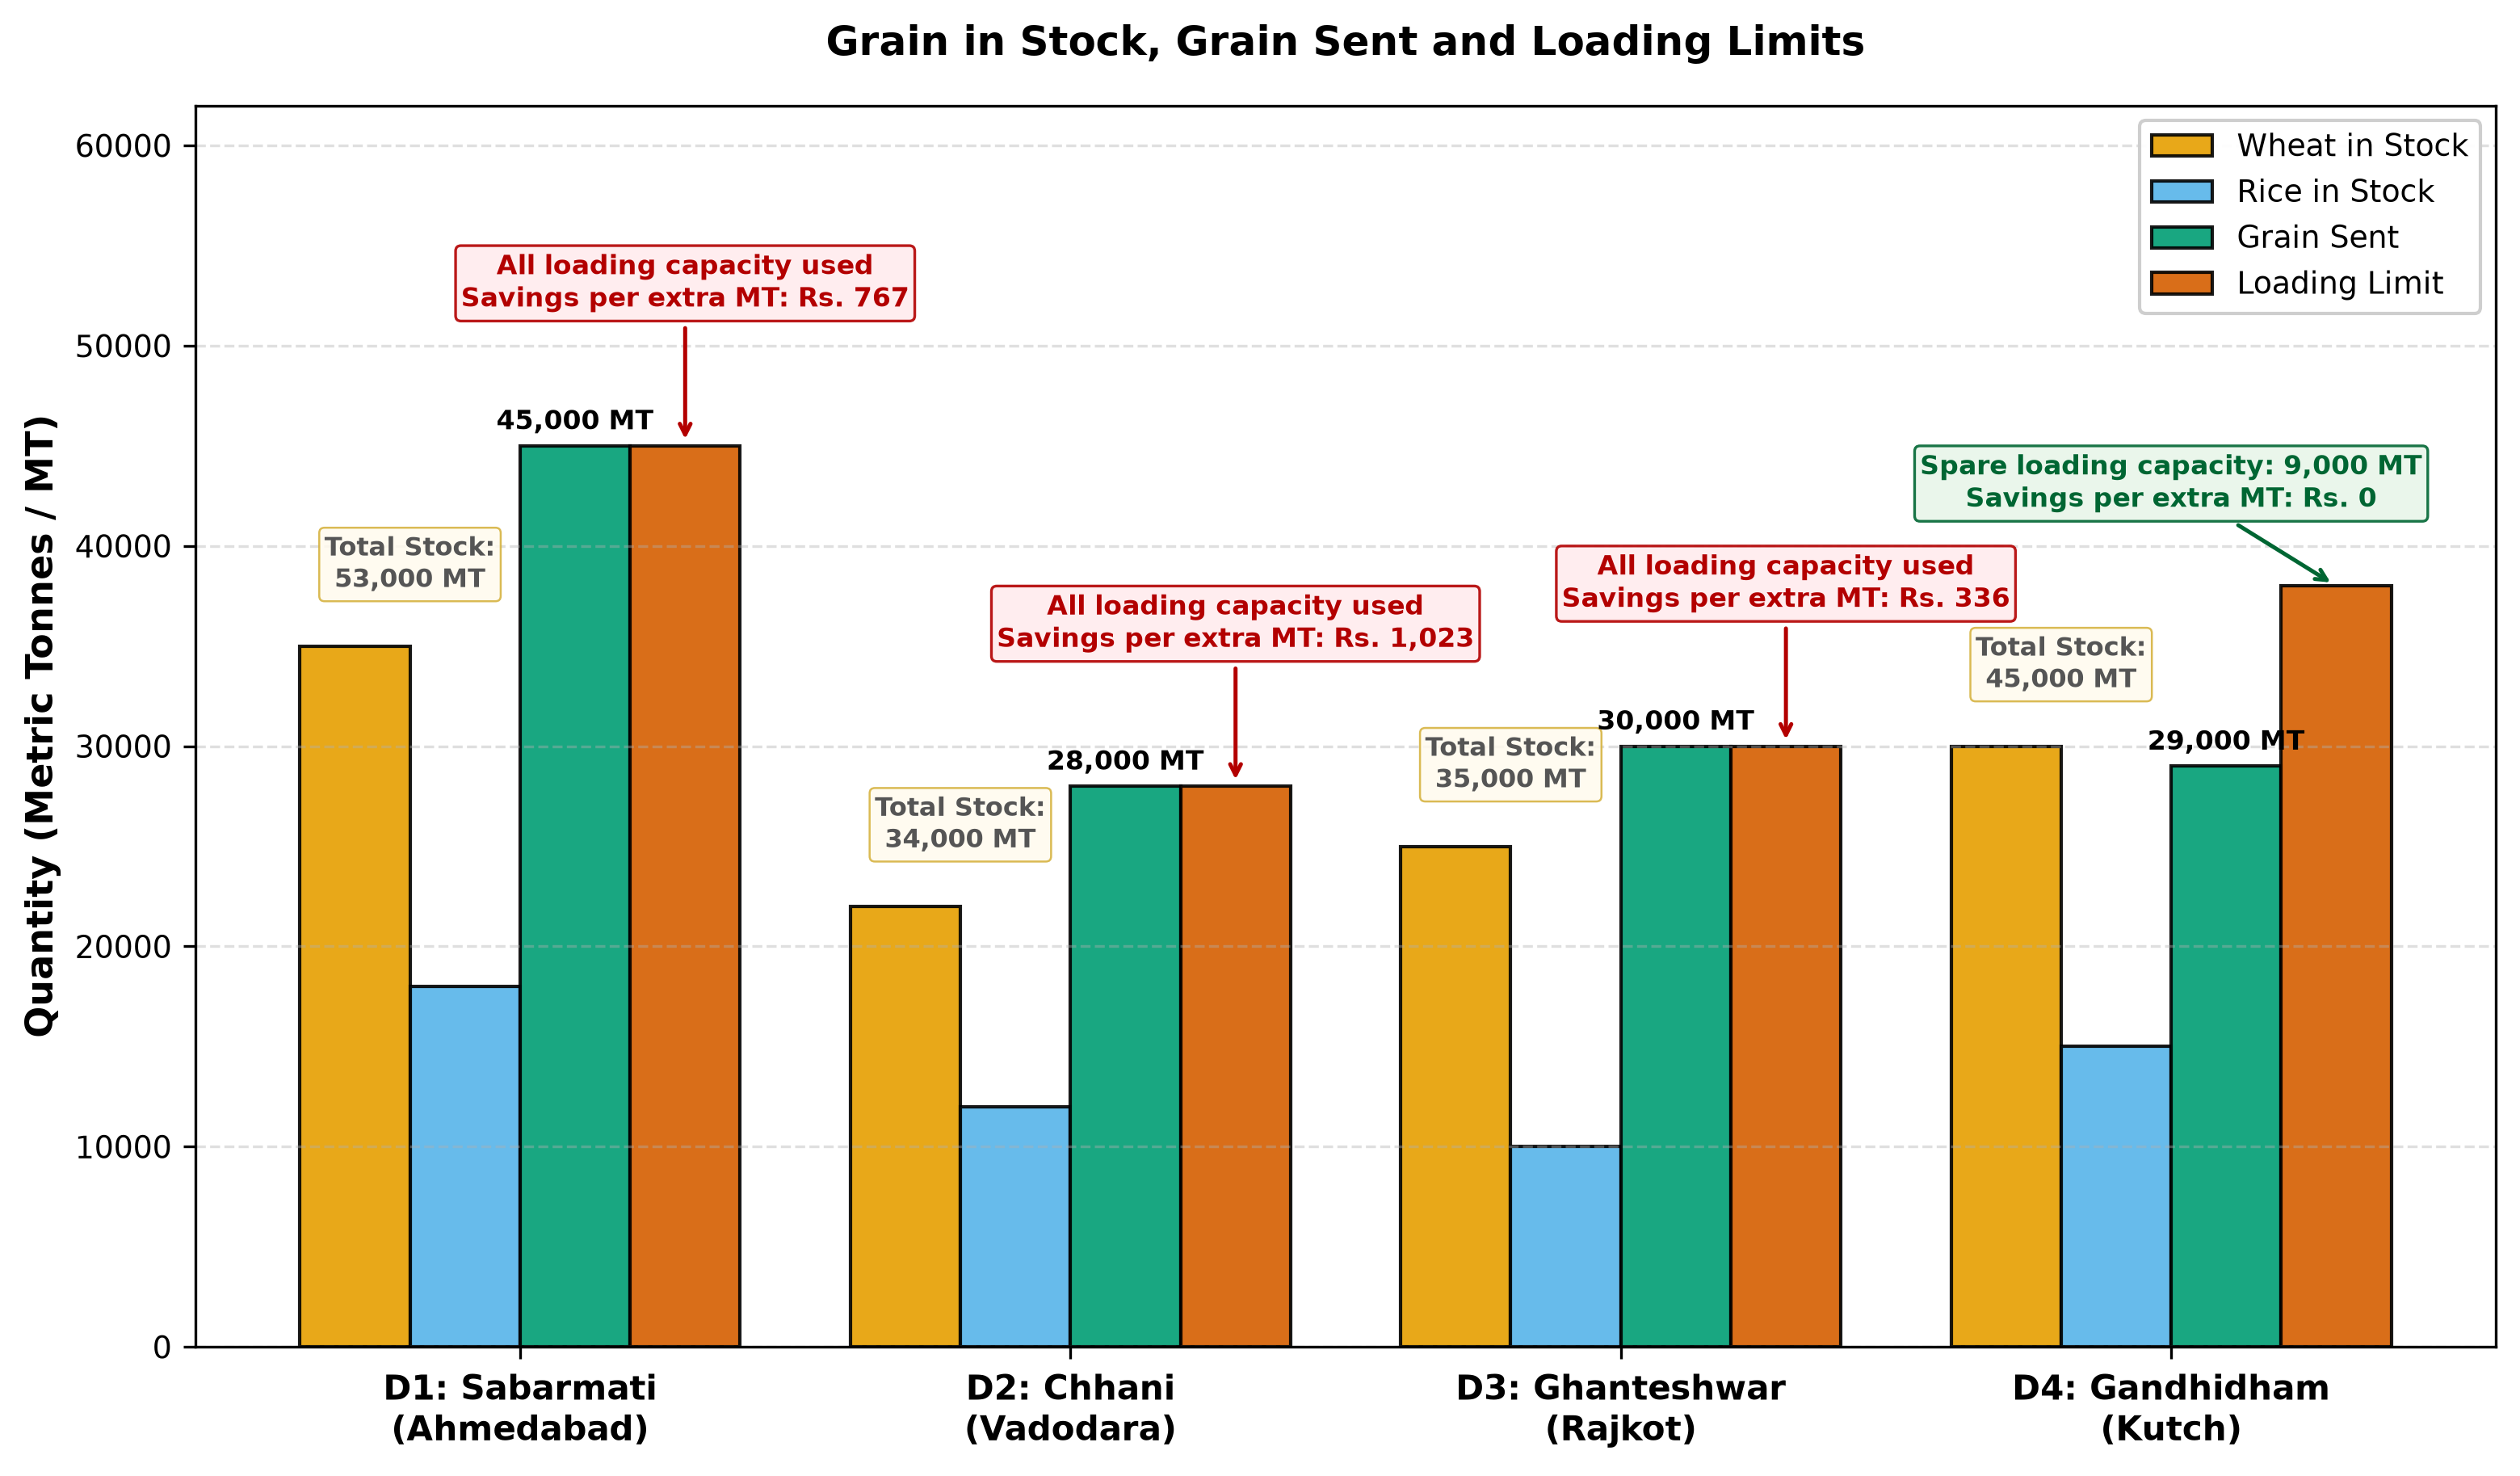
\includegraphics[width=\textwidth]{fig2_depot_utilization.png}\\
\vspace{-4pt}
\caption{\footnotesize Depot Stock vs.\ Dispatched Flow vs.\ Capacity ($C_i$).}
\end{minipage}
\end{figure}

\vspace{-6pt}


\subsection*{2. Why Surat Needs Grain from All Four Depots}
Surat needs 34,000 MT per month, made up of 22,000 MT of wheat and 12,000 MT of rice. There is no supply depot in Surat among the four we model. Chhani is the closest, about 155 km away, and its route to Surat costs Rs.~487.20 per tonne. Chhani sends 21,000 MT to nearby Vadodara, leaving just $28{,}000-21{,}000=7{,}000$ MT of monthly loading capacity for Surat.

Sabarmati sends 34,000 MT to Ahmedabad and uses the remaining 11,000 MT of its 45,000 MT limit for Surat. Ghanteshwar sends 18,000 MT to Rajkot and uses the remaining 12,000 MT of its 30,000 MT limit for Surat. Together with Chhani, these depots cover 30,000 MT of Surat's requirement and use all their loading capacity.

The remaining 4,000 MT comes from Gandhidham as rice, travelling about 564 km at Rs.~1,510.10 per tonne. This route alone costs Rs.~60.40 lakh per month. In the plan shown in Table 4.1, the four routes to Surat account for about 56\% of total transport and handling cost, even though Surat receives about 26\% of the grain. The longer trips illustrate why loading capacity near Surat matters.

\vfill
\begin{flushright}
\footnotesize \textit{Page 4 of 7}
\end{flushright}

\newpage

% ==============================================================================
% PAGE 5: SECTION 5 - ONE SENSITIVITY CHECK (10% Rubric Weight)
% ==============================================================================
\section*{Section 5: One Sensitivity Check}


\subsection*{1. Sensitivity Check: Expanding Chhani's Loading Capacity}
We solved the model with Chhani's monthly loading limit set to 21,000 through 35,000 MT in steps of 1,000 MT. The shadow price measures the cost saving from a small increase in loading capacity, in INR per MT. At a breakpoint, the savings can differ on either side.

\vspace{-4pt}
\textbf{Table 5.1: Parametric Sensitivity of FSD Chhani Dispatch Capacity ($C_2$)}
\begin{table}[h!]
\centering
\resizebox{\textwidth}{!}{
\begin{tabular}{ccccccc}
\toprule
\textbf{Chhani Cap $C_2$ (MT)} & \textbf{Total Cost (\Rs Cr)} & \textbf{Shadow Price $y_2^*$ (\INR/MT)} & \textbf{Chhani $\to$ Surat (MT)} & \textbf{Sabarmati $\to$ Surat (MT)} & \textbf{Gandhidham $\to$ Surat (MT)} & \textbf{Savings vs Baseline (\INR)} \\
\midrule
21,000 & \Rs 6.4143 Cr & \INR 1,022.90 & 0.0 & 11,000.0 & 11,000.0 & -\INR 7,160,300.00 \\
24,000 & \Rs 6.1074 Cr & \INR 1,022.90 & 3,000.0 & 11,000.0 & 8,000.0 & -\INR 4,091,600.00 \\
\textbf{28,000 (Base)} & \textbf{\Rs 5.6983 Cr} & \textbf{\INR 1,022.90} & \textbf{7,000.0} & \textbf{11,000.0} & \textbf{4,000.0} & \textbf{\INR 0.00} \\
30,000 & \Rs 5.4937 Cr & \INR 1,022.90 & 9,000.0 & 11,000.0 & 2,000.0 & +\INR 2,045,800.00 \\
31,000 & \Rs 5.3914 Cr & \INR 1,022.90 & 10,000.0 & 11,000.0 & 1,000.0 & +\INR 3,068,700.00 \\
32,000 & \Rs 5.2891 Cr & \INR 706.55 & 11,000.0 & 11,000.0 & 0.0 & +\INR 4,091,600.00 \\
\textbf{34,000 (Break)} & \textbf{\Rs 5.1478 Cr} & \textbf{\INR 706.55 $\to$ 0.00} & \textbf{13,000.0} & \textbf{9,000.0} & \textbf{0.0} & \textbf{+\INR 5,504,700.00} \\
\bottomrule
\end{tabular}
}
\end{table}

\vspace{-4pt}
\begin{figure}[h!]
\centering
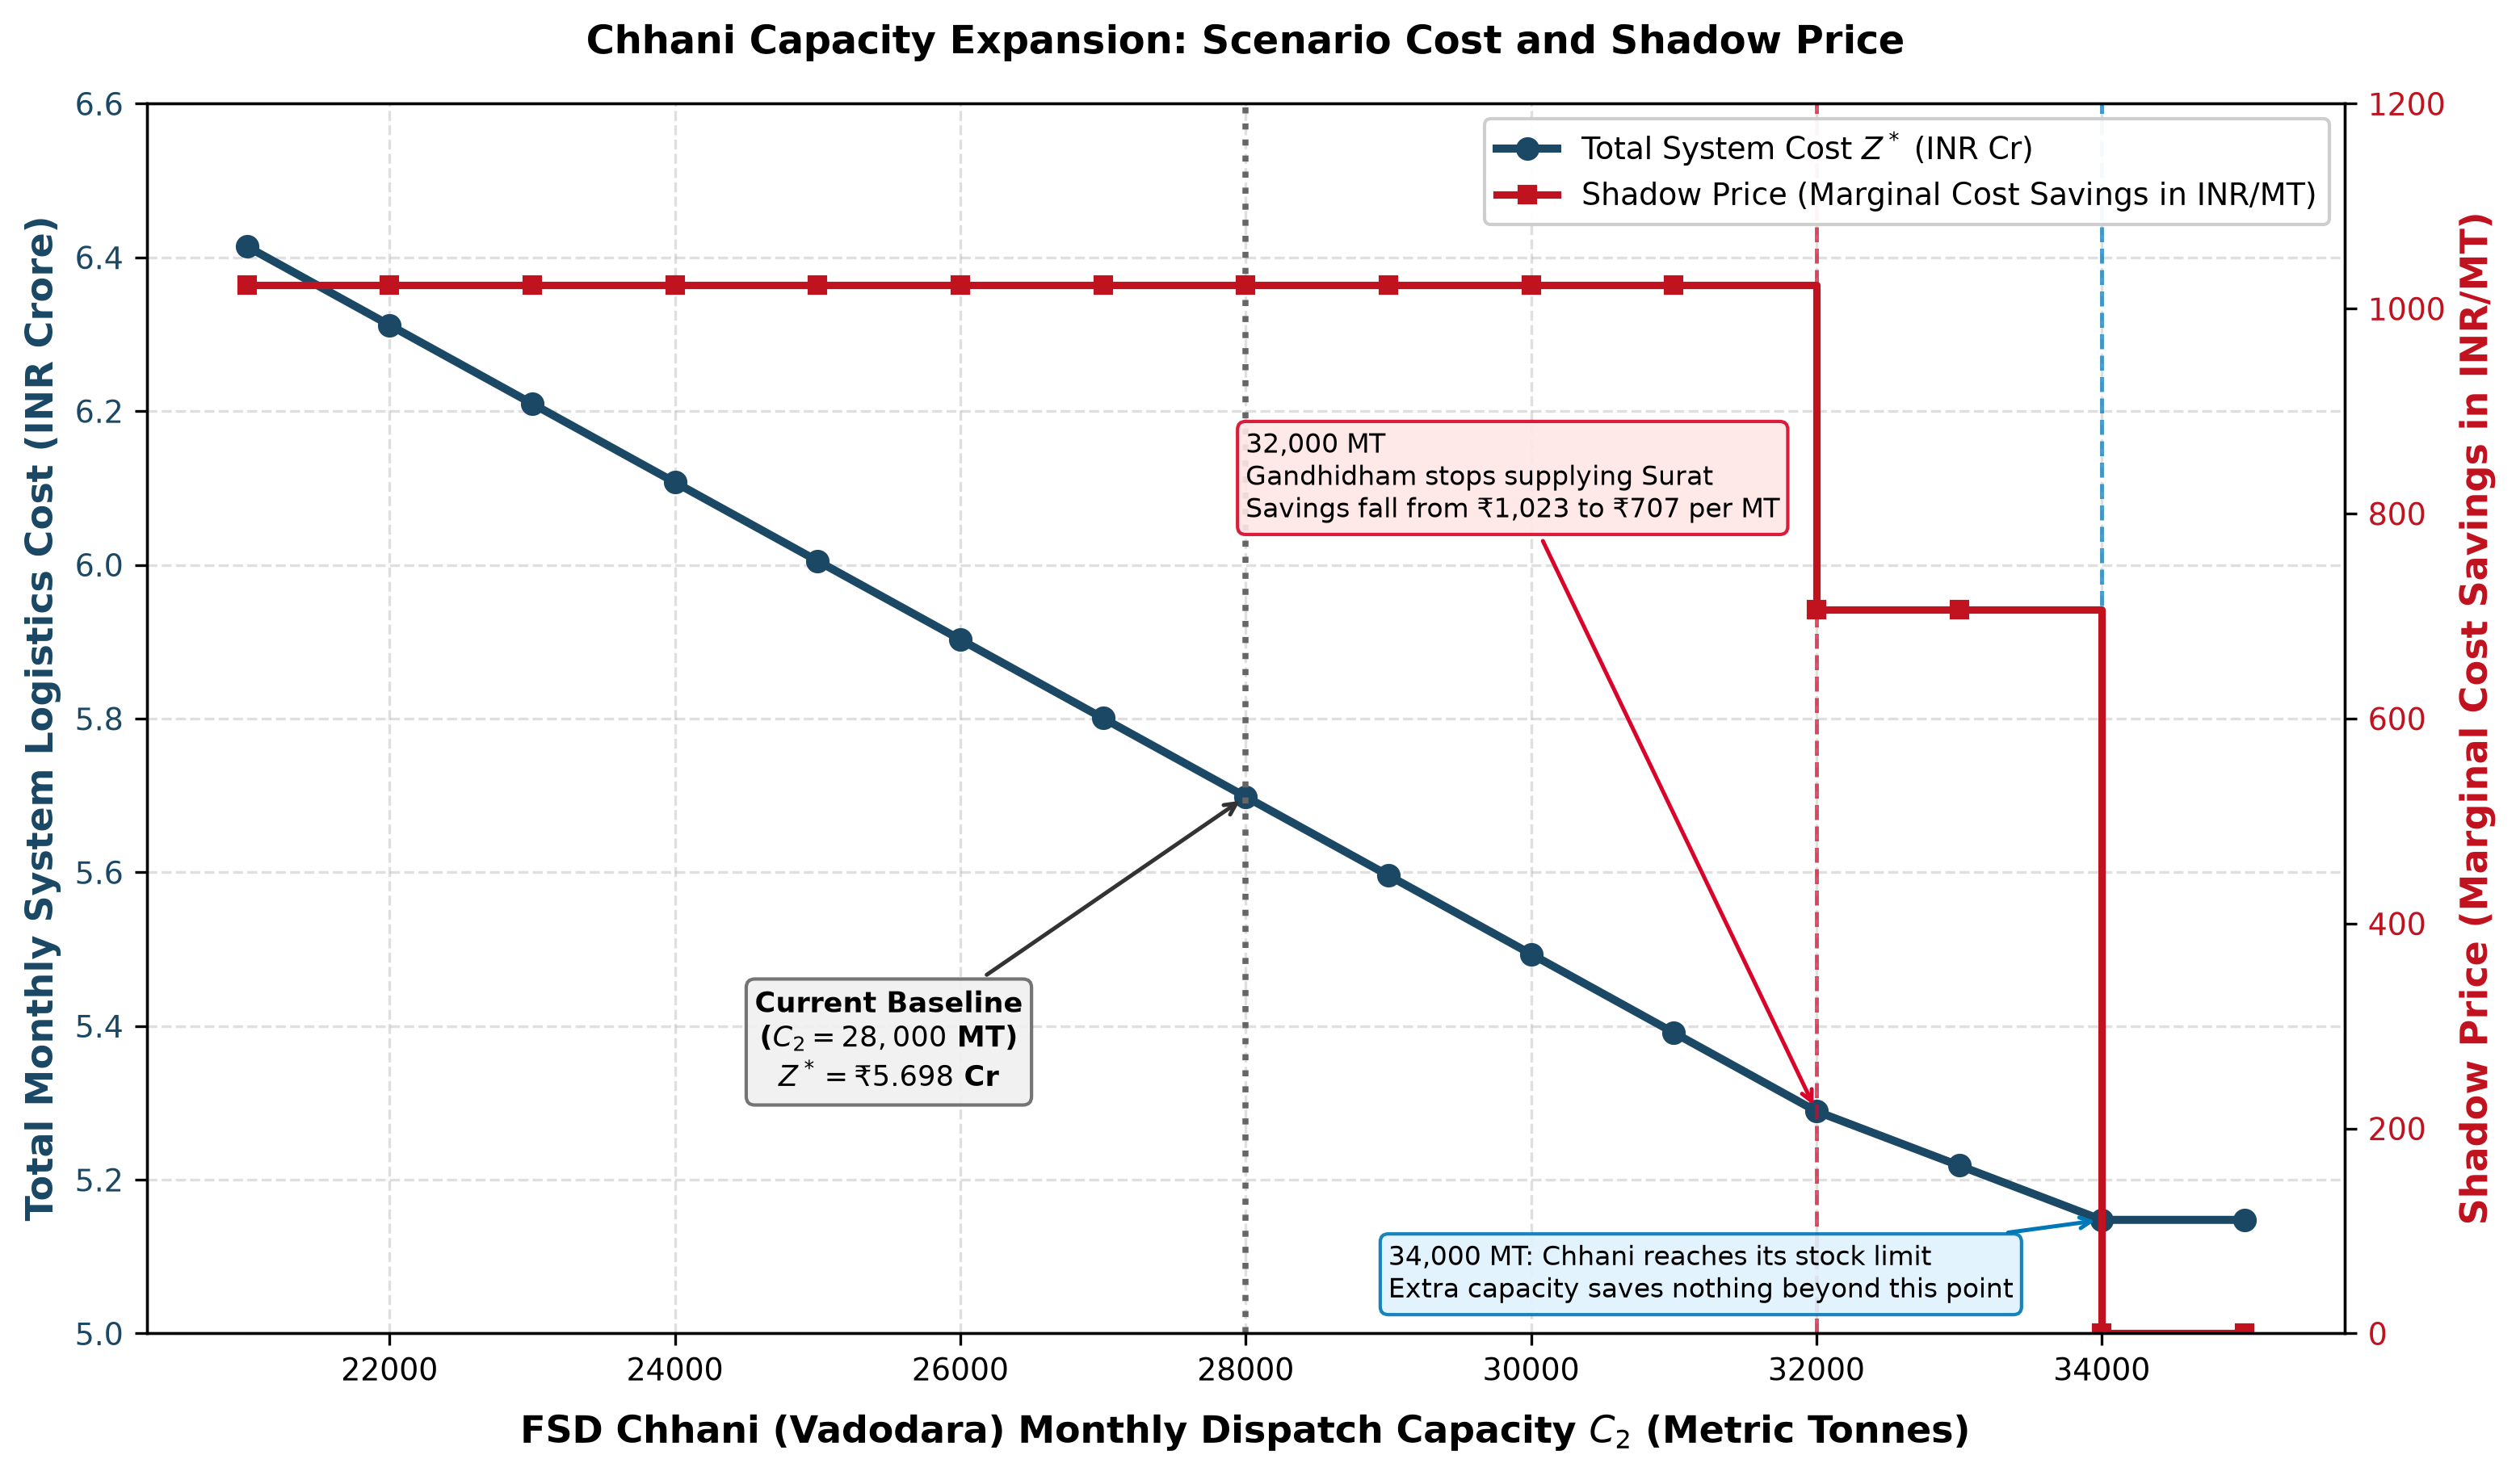
\includegraphics[width=0.72\textwidth]{fig3_sensitivity_curve_shadow_price.png}
\vspace{-4pt}
\caption{\footnotesize Effect of Chhani dispatch capacity on total transport cost and shadow price. The table reports the solver value at each limit. The curve shows savings for the next tonne, which fall to zero at 34,000 MT.}
\end{figure}

\vspace{-4pt}

\subsection*{2. Where the Savings Come From}
\textbf{Step 1 (28,000 to 32,000 MT --- Saving Rs.~1,022.90 per MT).}
For each extra tonne Chhani sends to Surat, Gandhidham sends one tonne less to Surat. The cost falls from Rs.~1,510.10 to Rs.~487.20 per tonne. The difference is Rs.~1,022.90, so the first 4,000 extra tonnes save \textbf{Rs.~40,91,600 per month}.

\textbf{Step 2 (32,000 to 34,000 MT --- Saving Rs.~706.55 per MT).}
Chhani takes over another tonne for Surat from Sabarmati, saving Rs.~743.55 minus Rs.~487.20, or Rs.~256.35. Sabarmati can now send a tonne to Banaskantha in place of Gandhidham, saving Rs.~900.70 minus Rs.~450.50, or Rs.~450.20. Together these changes save Rs.~706.55 per tonne. The next 2,000 tonnes save \textbf{Rs.~14,13,100 per month}.

The two steps save \textbf{INR 5,504,700.00 per month} (Rs.~55.05 lakh), or about \textbf{Rs.~6.61 Crore} in a year if the same demand and costs hold. Adding loading capacity beyond 34,000 MT saves nothing because Chhani has no more grain to send.

\subsection*{3. What If the Rate per Kilometre Changes?}
We tested rates from Rs.~1.50 to Rs.~4.00 per tonne-km. Total cost rose roughly in a straight line, and the routes used stayed the same.

\vfill
\begin{flushright}
\footnotesize \textit{Page 5 of 7}
\end{flushright}

\newpage

% ==============================================================================
% PAGE 6: SECTION 6 - WHAT THE MODEL CANNOT SAY (10% Rubric Weight)
% ==============================================================================
\section*{Section 6: What the Model Cannot Say}


\begin{enumerate}\setlength{\itemsep}{16pt}\large
\item The model treats shipments as continuous quantities, so it does not count whole truckloads or charge for empty return trips, both of which can affect the actual cost of a schedule when, for example, a 26 MT shipment needs two trips with a truck that carries at most 25 MT.

\item By grouping demand at six district headquarters, the model estimates the cost of moving bulk grain to each district but leaves out the second leg to taluka godowns and Fair Price Shops, where the number of stops, smaller loads and local road conditions would affect both cost and delivery time.

\item The model uses a single average month, so it does not track how harvest peaks change available stock, how monsoon disruptions change road access, or how grain carried into later months can spoil, all of which matter when planning stock levels and deliveries across a year.
\end{enumerate}

\vfill
\begin{flushright}
\footnotesize \textit{Page 6 of 7}
\end{flushright}

\newpage

% ==============================================================================
% PAGE 7: REFERENCES
% ==============================================================================
\section*{References}

\begin{enumerate}\setlength{\itemsep}{10pt}
\item \textbf{Department of Food \& Public Distribution (DFPD), Government of India}. \textit{National Food Security Act (NFSA) 2013: Coverage and Entitlements (Priority Households \& Antyodaya Anna Yojana)}. \url{https://www.nfsa.gov.in/portal/Coverage_Entitlements_NFSA_AA}. Accessed 7 November 2026.
\item \textbf{Food Corporation of India (FCI) Gujarat Regional Office \& Directorate of Food and Civil Supplies, Government of Gujarat}. \textit{District-wise Storage Godown Capacities and Monthly PDS Allocation Statistics}. \url{https://dcs-dof.gujarat.gov.in/} and \url{https://ipds.gujarat.gov.in/}. Accessed November 2026.
\item \textbf{Project OSRM}. \textit{Open Source Routing Machine: Distance Table API and High-Performance Routing Engine}. \url{https://project-osrm.org/docs/v5.24.0/api/#table-service}.
\item \textbf{Virtanen, P., Gommers, R., Oliphant, T. E., et al.} (2020). SciPy 1.0: Fundamental Algorithms for Scientific Computing in Python. \textit{Nature Methods}, 17(3), 261--272. HiGHS Linear Optimization Solver: \url{https://docs.scipy.org/doc/scipy/reference/optimize.linprog-highs-ds.html}.
\item \textbf{Project Repository \& Implementation Code}. Optimization pipelines, Two-Phase Simplex solvers, and datasets in \texttt{scripts/01}--\texttt{scripts/05}, \texttt{data/}, and \texttt{outputs/tables/}. IIT Gandhinagar.
\end{enumerate}

\vfill
\begin{flushright}
\footnotesize \textit{Page 7 of 7}
\end{flushright}



\end{document}
